
\documentclass{article}
\usepackage[]{tikz}

\begin{document}
    
\begin{tikzpicture}
    \path (0,2) node [shape=circle,draw] {}
        (0,1) node [shape=circle,draw] {}
        (0,0) node [shape=circle,draw] {}
        (1,1) node [shape=rectangle,draw] {}
        (-1,1) node [shape=rectangle,draw] {};
\end{tikzpicture}

\begin{tikzpicture}
    \node at (0,2) [circle,draw] {};
    \node at (0,1) [circle,draw] {};
    \node at (0,0) [circle,draw] {};
    \node at (1,1) [rectangle,draw] {};
    \node at (-1,1) [rectangle,draw] {};
\end{tikzpicture}

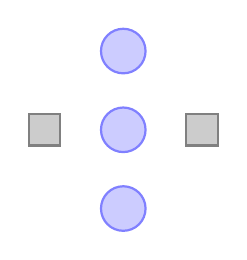
\begin{tikzpicture}
    [
        inner sep=2mm,
        place/.style={circle, draw=blue!50, fill=blue!20, thick},
        transition/.style={rectangle, draw=black!50, fill=black!20, thick}
    ]
    \node at (0,2) [place] {};
    \node at (0,1) [place] {};
    \node at (0,0) [place] {};
    \node at (1,1) [transition] {};
    \node at (-1,1) [transition] {};
\end{tikzpicture}
\end{document}
